\documentclass[14pt,a4paper,report]{report}
\usepackage[a4paper, mag=1000, left=2.5cm, right=1cm, top=2cm, bottom=2cm, headsep=0.7cm, footskip=1cm]{geometry}
\usepackage[utf8]{inputenc}
\usepackage[english,russian]{babel}
\usepackage{indentfirst}
\usepackage[dvipsnames]{xcolor}
\usepackage[colorlinks]{hyperref}
\usepackage{listings} 
\usepackage{fancyhdr}
\usepackage{caption}
\usepackage{amsmath}
\usepackage{latexsym}
\usepackage{graphicx}
\hypersetup{
	colorlinks = true,
	linkcolor  = black
}

\usepackage{titlesec}
\titleformat{\chapter}
{\Large\bfseries} % format
{}                % label
{0pt}             % sep
{\huge}           % before-code


\DeclareCaptionFont{white}{\color{white}} 

% Listing description
\usepackage{listings} 
\DeclareCaptionFormat{listing}{\colorbox{gray}{\parbox{\textwidth}{#1#2#3}}}
\captionsetup[lstlisting]{format=listing,labelfont=white,textfont=white}
\lstset{ 
	% Listing settings
	inputencoding = utf8,			
	extendedchars = \true, 
	keepspaces = true, 			  	 % Поддержка кириллицы и пробелов в комментариях
	language = Matlab,            	 	 % Язык программирования (для подсветки)
	basicstyle = \small\sffamily, 	 % Размер и начертание шрифта для подсветки кода
	numbers = left,               	 % Где поставить нумерацию строк (слева\справа)
	numberstyle = \tiny,          	 % Размер шрифта для номеров строк
	stepnumber = 1,               	 % Размер шага между двумя номерами строк
	numbersep = 5pt,              	 % Как далеко отстоят номера строк от подсвечиваемого кода
	backgroundcolor = \color{white}, % Цвет фона подсветки - используем \usepackage{color}
	showspaces = false,           	 % Показывать или нет пробелы специальными отступами
	showstringspaces = false,    	 % Показывать или нет пробелы в строках
	showtabs = false,           	 % Показывать или нет табуляцию в строках
	frame = single,              	 % Рисовать рамку вокруг кода
	tabsize = 2,                  	 % Размер табуляции по умолчанию равен 2 пробелам
	captionpos = t,             	 % Позиция заголовка вверху [t] или внизу [b] 
	breaklines = true,           	 % Автоматически переносить строки (да\нет)
	breakatwhitespace = false,   	 % Переносить строки только если есть пробел
	escapeinside = {\%*}{*)}      	 % Если нужно добавить комментарии в коде
}

\begin{document}

\def\contentsname{Содержание}

% Titlepage
\begin{titlepage}
	\begin{center}
		\textsc{Санкт-Петербургский Политехнический 
			Университет Петра Великого\\[5mm]
			Кафедра компьютерных систем и программных технологий}
		
		\vfill
		
		\textbf{Отчёт по лабораторной работе №1\\[3mm]
			Курс: «Теория автоматического управления»\\[41mm]
			}
	\end{center}
	
	\hfill
	\begin{minipage}{.5\textwidth}
		Выполнил студент:\\[2mm] 
		Бояркин Никита Сергеевич\\
		Группа: 43501/3\\[5mm]
		
		Проверил:\\[2mm] 
		Нестеров Сергей Александрович
	\end{minipage}
	\vfill
	\begin{center}
		Санкт-Петербург\\ \the\year\ г.
	\end{center}
\end{titlepage}

% Contents
\tableofcontents
\clearpage

\chapter{Лабораторная работа №1}

\section{Цель работы}

Получение навыков по построению всех форм математических моделей, временных и частотных характеристик.

\section{Программа работы}

\begin{itemize}
	\item Получить передаточную функцию.
	\item Решить ДУ.
	\item Получить частотные характеристики Найквиста и Боде.
	\item Получить переходную и весовую временные характеристики.
	\item Получить фазовую траекторию.
\end{itemize}

\section{Индивидуальное задание}

$x''+25x'=5u'+25u, x(0)=0, x'(0)=0, u=1(t)$

\section{Ход работы}

\subsection{Получение передаточной функции}

Уравнение уже приведено в линейный вид, следовательно можно сразу воспользоваться преобразованием Лапласа и получить передаточную функцию:

$
\\
x''+25x'=5u'+25u\\
xp^2+25xp=5up+25u \\
x(p^2+25p)=u(5p+25) \\
W(p)=\frac{x}{u}=\frac{5p+25}{p^2+25p}\\
$

Добавим входное воздействие, передаточную функцию и выходное воздействие на ВВ модель:

\begin{figure}[h!]
	\centering
	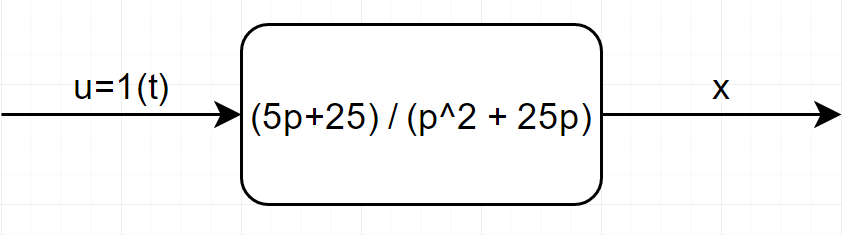
\includegraphics[scale = 0.55]{images/ou.png}
	\caption{ВВ модель}
	\label{image:1}
\end{figure}

\clearpage

Подберем электрическую цепь, которая обеспечивает заданную передаточную характеристику:

\begin{figure}[h!]
	\centering
	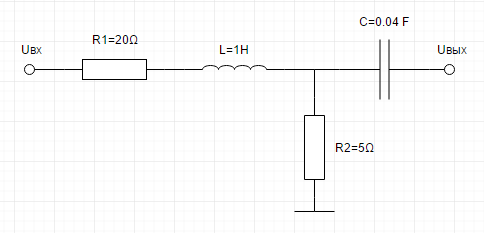
\includegraphics[scale = 0.79]{images/schema.png}
	\caption{Пример электрической цепи для заданной передаточной функции}
	\label{image:2}
\end{figure}

$
\\
Uвх=I(R_1+Lp+R_2)\\
Uвых=I(\frac{1}{Cp}+R_2)\\
W(p)=\frac{U_{out}}{U_{in}}=\frac{I(\frac{1}{Cp}+R_2)}{I(R_1+Lp+R_2)}=\frac{\frac{1}{C}+R_2p}{R1p+Lp^2+R2p}=\frac{\frac{1}{0.04}+5p}{20p+1p^2+5p}=\frac{5p+25}{p^2+25p}\\
$

\subsection{Решение дифференциального уравнения}

\begin{equation*}
	\text{$u=1(t)=$}
	\begin{cases}
		\text{$1, t\geq0$} \\
		\text{$0, t<0$}
	\end{cases}
	\Longrightarrow
	\text{$u'=\delta(t)=$}
	\begin{cases}
		\text{$\infty, t=0$} \\
		\text{$0, t\neq0$}
	\end{cases}
\end{equation*}

\begin{equation*}
	\text{$x''+25x'=$}
	\begin{cases}
		\text{$5\cdot0+25\cdot0, t<0$} \\
		\text{$5\cdot\infty+25\cdot1, t=0$} \\
		\text{$5\cdot0+25\cdot1, t>0$} \\
	\end{cases}
	\text{$=$}
	\begin{cases}
		\text{$0, t<0$} \\
		\text{$\infty, t=0$} \\
		\text{$25, t>0$} \\
	\end{cases}
\end{equation*}

Таким образом имеется три участка кусочной функции для решения ДУ. При $t=0$ ДУ уже решено (по начальным условиям $x(0)=0, x'(0)=0 => x''(0)=\infty$).

Решим ДУ для случая $t<0$ с помощью Matlab функции $dsolve$:

\begin{lstlisting}
syms x(t) dx(t)
x(t) = dsolve(diff(x, t, 2) + 25 * diff(x, t) == 0)
\end{lstlisting}

В результате было получено:

$x(t<0)=C_1e^{-25t}+C_2 => x'(t<0)=-25C_1e^{-25t}$

Аналогичным образом решим ДУ для случая $t>0$:

\begin{lstlisting}
syms x(t) dx(t)
x(t) = dsolve(diff(x, t, 2) + 25 * diff(x, t) == 25)
\end{lstlisting}

В результате было получено:

$x(t>0)=C_1e^{-25t}+C_2+t => x'(t>0)=1-25C_1e^{-25t}$

Важно отметить, что пограничный случай $t=0, x(0)=0$ можно отнести как и к результату при $t<0$, если $C_1=0, C_2=0$, так и к $t>0$ при тех же константах. Это означает, что функция $x(t)$ непрерывна в этой точке.

\subsection{Частотные характеристики}

$
\\
W(jf)=\frac{5jf+25}{25jf-f^2}=\frac{(5jf+25)(25jf+f^2)}{(25jf-f^2)(25jf+f^2)}=\frac{-125f^2+625jf+5jf^3+25f^2}{-625f^2-f^4}=\frac{100f-(625+5f^2)j}{625f+f^3}=\frac{100}{625+f^2}-\frac{625+5f^2}{625f+f^3}j$

$
\\
u(f)=real(W(jf))=\frac{100}{625+f^2}\\
v(f)=imagine(W(jf))=-\frac{625+5f^2}{625f+f^3}\\
A(f)=\sqrt{u^2(f) + v^2(f)}\\
\alpha(f)=20lgA(f)\\
$

\clearpage

Построим диаграмму Найквиста с помощью Matlab функции $nyquist$:

\begin{figure}[h!]
	\centering
	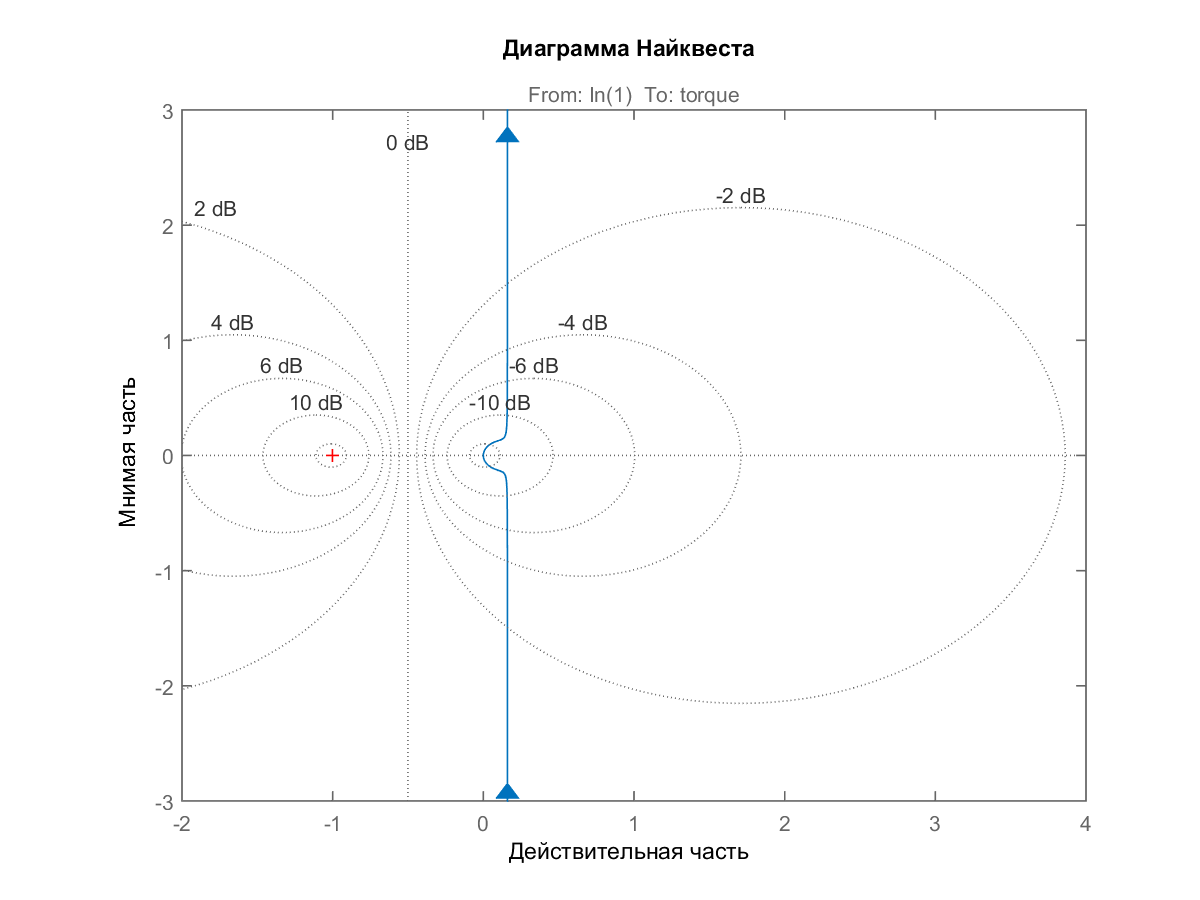
\includegraphics[scale = 0.70]{images/nyquist.png}
	\caption{Диаграмма Найквиста}
	\label{image:3}
\end{figure}

Построим диаграмму Боде с помощью Matlab функции $bode$:

\begin{figure}[h!]
	\centering
	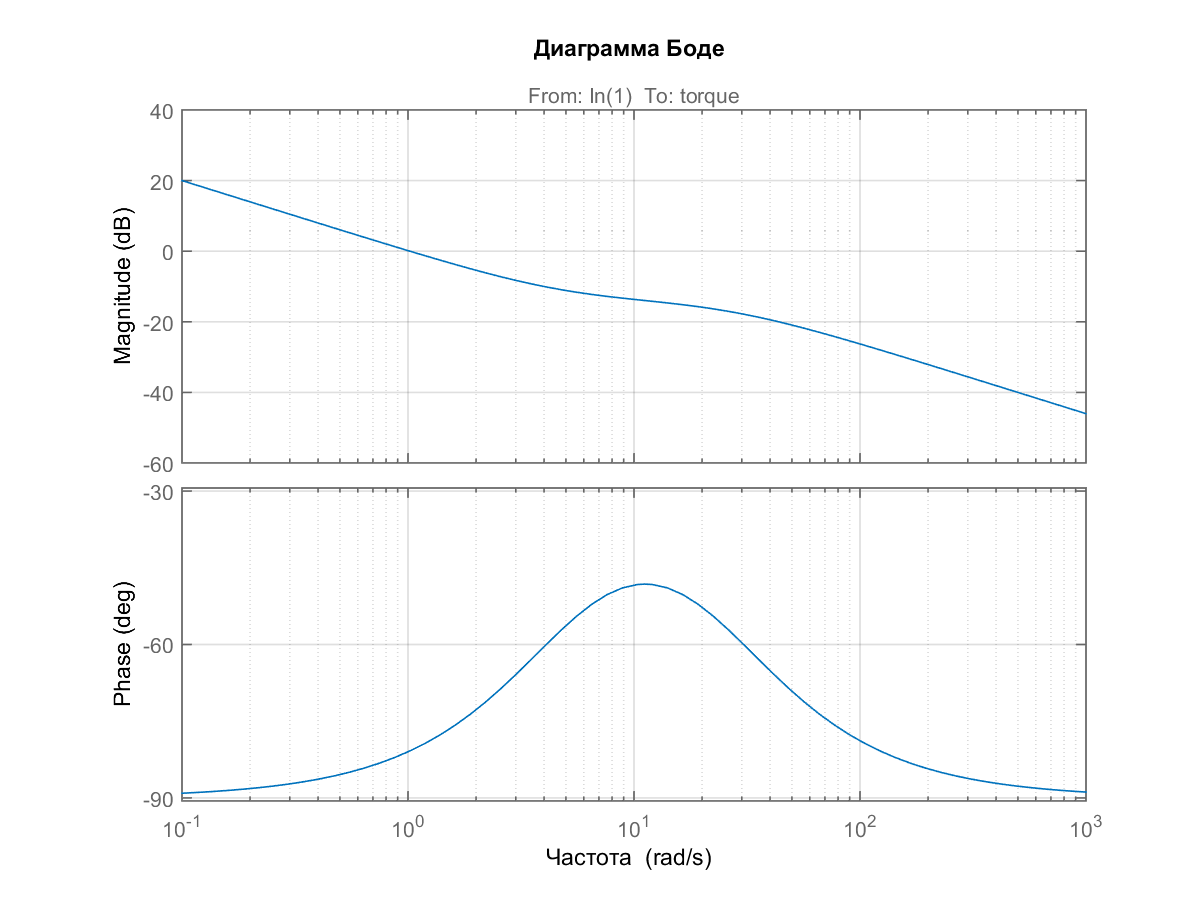
\includegraphics[scale = 0.70]{images/bode.png}
	\caption{Диаграмма Боде}
	\label{image:4}
\end{figure}

\subsection{Временные характеристики}

$
\\
h(t)=L^{-1}(\frac{W(p)}{p})=L^{-1}(\frac{5p+25}{p^2(p+25)})=L^{-1}(\frac{1}{p^2}-\frac{0.16}{p+25}+\frac{0.16}{p})=t+0.16-0.16e^{-25t}\\
w(t)=\frac{dh(t)}{dt}=1+4e^{-25t}\\
$

Построим переходную характеристика с помощью Matlab функции $step$:

\begin{figure}[h!]
	\centering
	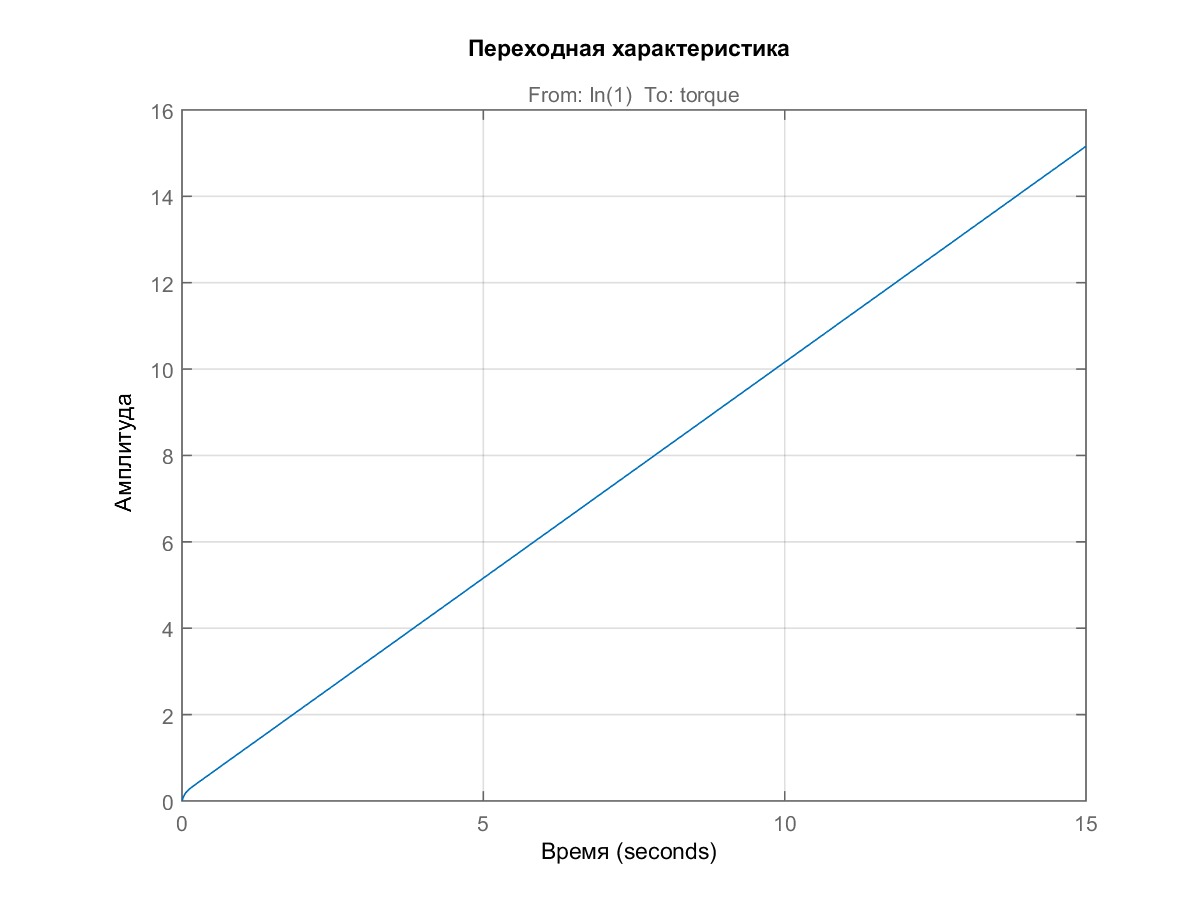
\includegraphics[scale = 0.60]{images/step.png}
	\caption{Переходная характеристика}
	\label{image:5}
\end{figure}

Построим весовую характеристика с помощью Matlab функции $impulse$:

\begin{figure}[h!]
	\centering
	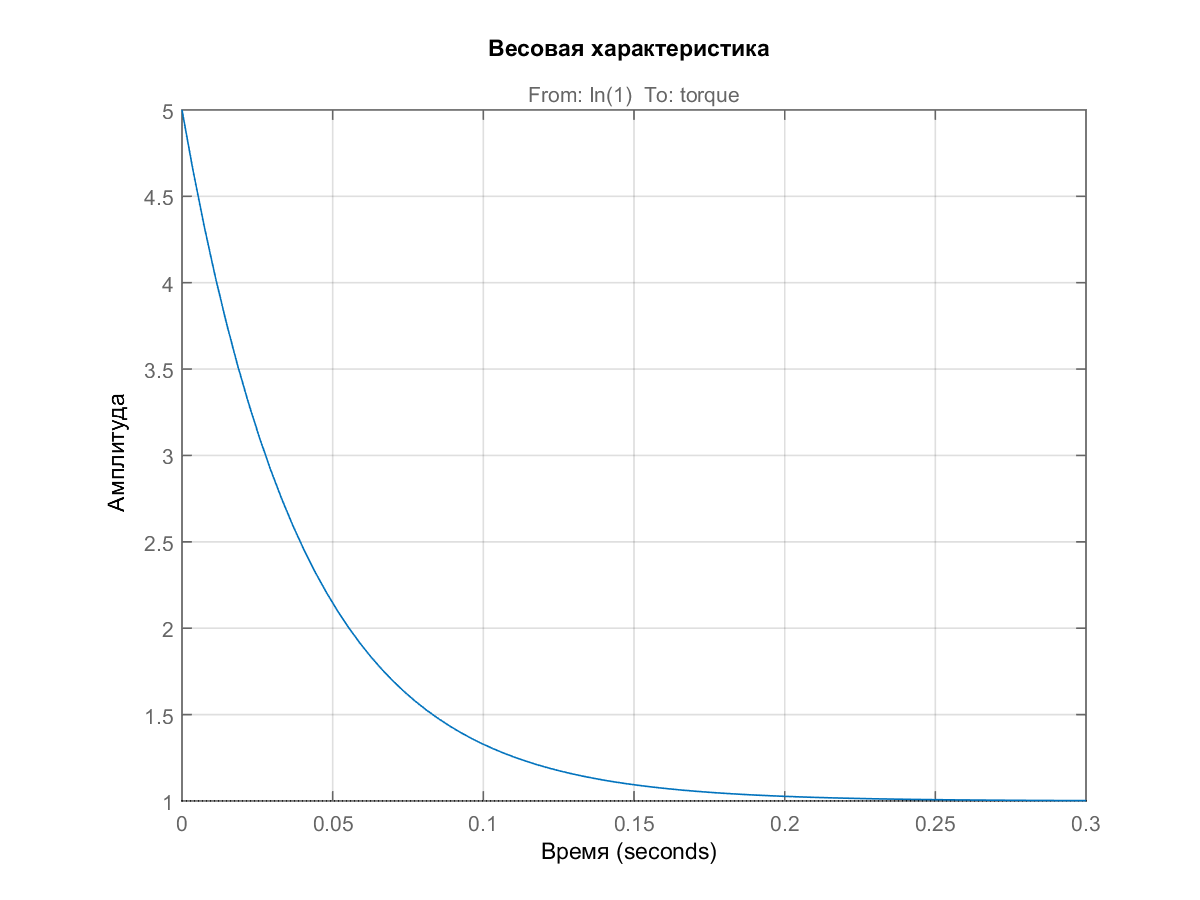
\includegraphics[scale = 0.60]{images/impulse.png}
	\caption{Весовая характеристика}
	\label{image:6}
\end{figure}

\subsection{Фазовый портрет}

Выполним замену переменной:

$Y=x'(t), X=x(t)$

%Тогда ДУ преобразовывается к следующей системе (в точке $t=0$ функция непрерывна, поэтому можно отнести ее к случаю $t\leq0$):

Тогда ДУ преобразовывается к следующей системе:

\begin{equation*}
%	\text{$x''+25x'=$}
	\text{$x''+25x'=0$}
%	\begin{cases}
%		\text{$0, t<0$} \\
%		\text{$\infty, t=0$} \\
%		\text{$25, t>0$} \\
%	\end{cases}
	\Longrightarrow
	\begin{cases}
		\text{$Y'=-25Y$} \\
%		\begin{cases}
%			\text{$Y'=-25Y, t\leq0$} \\
%			\text{$Y'=25-25Y, t>0$} \\
%		\end{cases} \\
		\text{$X'=Y$} \\
	\end{cases}
\end{equation*}

После этого преобразования можно рассчитать фазовый портрет системы. Расчет численных значений $x(t)$ и $x'(t)$ производится с помощью Matlab функции $ode45$:

%\begin{figure}[h!]
%	\centering
%	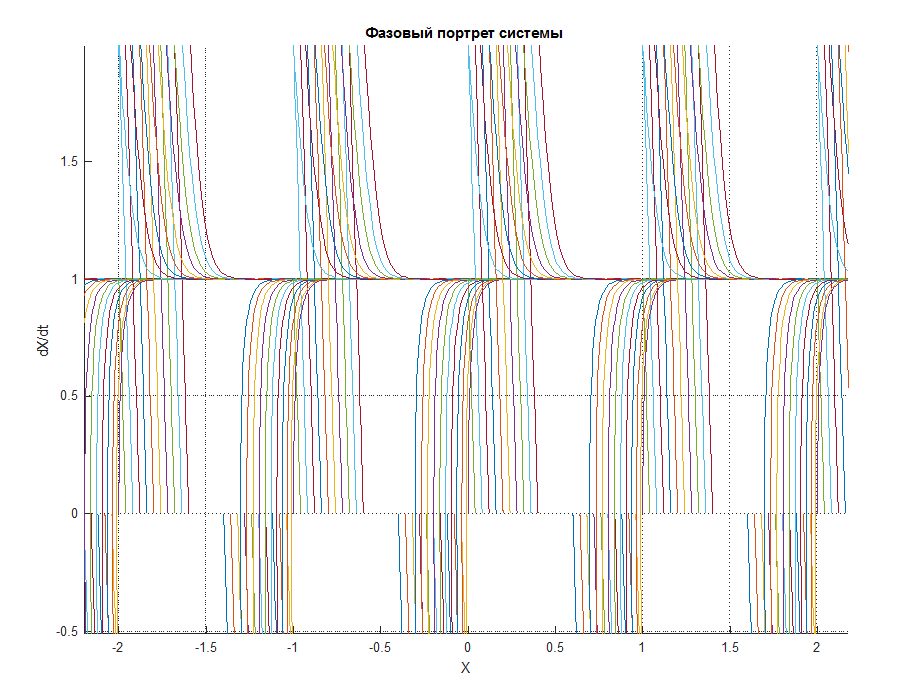
\includegraphics[scale = 0.43]{images/odezoom.png}
%	\caption{Фазовый портрет системы}
%	\label{image:8}
%\end{figure}

%На графиках фазовых портретов хорошо видно, как часть графика при $t\leq0$ накладывается часть графика при $t>0$. 

%Для наглядности отобразим только часть графика, где $t\leq0$:

\begin{figure}[h!]
	\centering
	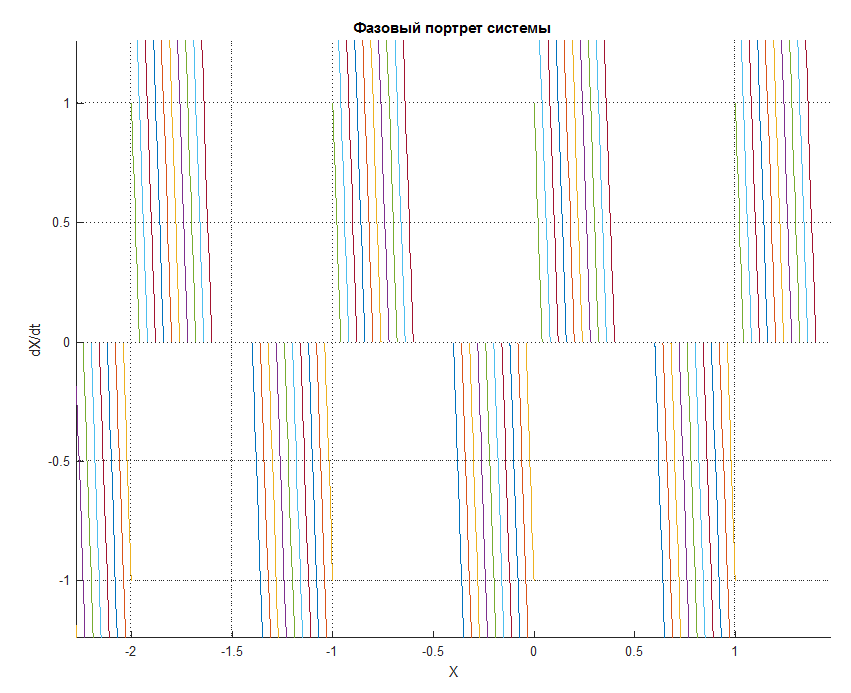
\includegraphics[scale = 0.43]{images/odeneg.png}
	%\caption{Фазовый портрет системы при $t\leq0$}
	\caption{Фазовый портрет системы}
	\label{image:9}
\end{figure}

Из графика хорошо видно, что фазовые траектории представляют собой прямые линии, докажем это. Заметим, что $F(x'',x',x)=0$ эквивалентно случаю $x(t\leq0)$. В результате решения ДУ было получено:

$x(t\leq0)=C_1e^{-25t}+C_2 => x'(t\leq0)=-25C_1e^{-25t}$

Таким образом:

$x'(t\leq0)=25C_2-25x(t\leq0)$

Тангенс наклона прямых линий равен $tg(k)=-25$.

%Рассмотрим часть графика, где $t>0$:

%\begin{figure}[h!]
%	\centering
%	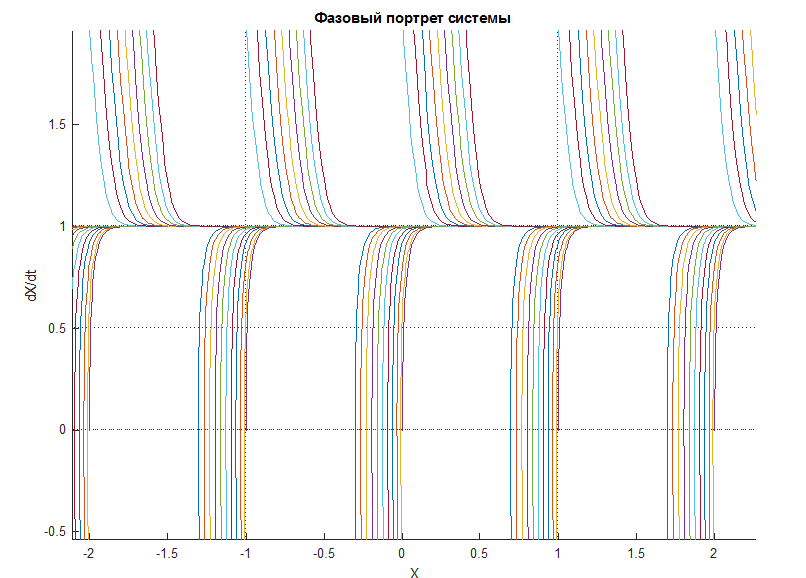
\includegraphics[scale = 0.48]{images/odepos.png}
%	\caption{Фазовый портрет системы при $t>0$}
%	\label{image:10}
%\end{figure}

%В результате решения ДУ было получено:

%$x(t>0)=C_1e^{-25t}+C_2+t => x'(t>0)=1-25C_1e^{-25t}$

%В этом случае не получится выразить $x'(x(t>0))$ поэтому тип фазового портрета неопределен.

\section{Вывод}

В ходе работы были получены важнейшие функции и характеристики для системы, заданной линейным ДУ и начальными условиями:

\begin{itemize}
	\item \emph{Диаграмма Найквиста (АФЧХ)} - представление частотного отклика линейной стационарной динамической системы в виде графика в комплексных координатах. АФЧХ применяется в основном для анализа систем, в частности исследования системы на устойчивость и её запасов.
	\item \emph{Диаграмма Боде (ЛАФЧХ)} - представление частотного отклика линейной стационарной системы в логарифмическом масштабе.
	\item \emph{Переходная функция} - реакция динамической системы на входное воздействие в виде функции Хевисайда. Знание того, как система реагирует на быстрое изменение входного сигнала, является важным, поскольку скачок во входном сигнале может оказать серьёзное влияние на поведение всей системы или каких-то её компонентов.
	\item \emph{Весовая функция} - реакция динамической системы на входное воздействие в виде единичного импульса. 
	\item \emph{Фазовый портрет} - Построение фазового портрета позволяет сделать выводы о характере изменений переменных системы без знания аналитических решений исходной системы уравнений.
\end{itemize}

Благодаря множеству плагинов, математических функций и методов симуляции, Matlab отлично подходит для решения задач, связанных с ТАУ.

\end{document}